<<<<<<< HEAD
\documentclass[12pt]{article}
\usepackage{amsmath,amssymb}
\usepackage[margin=0.5in]{geometry}
=======
\documentclass[11pt,preprint]{aastex}
\usepackage{amsmath,amssymb}
\usepackage{natbib}
>>>>>>> d9dbc942e0a1dc3bc215bd232df3eaebc4a33de1
\usepackage{graphicx} 
\begin{document}

\shorttitle{Mass Mapping A2261 with Kinematic Weak Lensing}
\shortauthors{Schlegel, et al.}

\section{Science Justification}
<<<<<<< HEAD
\noindent {\bf Weak Lensing with the Tully-Fisher Relation.} Weak gravitational lensing has been widely touted as a powerful probe of cosmology. It is a major science driver for several large imaging surveys, such as the Dark Energy Survey (DES) the Large Synoptic Survey Telescope (LSST), and space missions such as Euclid and the Wide-Field Infrared Survey Telescope (WFIRST). Weak lensing is weak, however, and all current measurements are limited by the scatter in galaxy shapes, which is an order of magnitude or more greater than the typical weak lensing signal. 
%This means that weak lensing analyses must average over every available galaxy image, pushing the analysis to include faint and poorly-resolved galaxies for which unbiased measurements of galaxy shapes are difficult. Precision estimates of galaxy redshifts from photometry is crucial for these analyses, as the current generation of ongoing surveys will entail sample sizes of a few $\times10^8$ galaxies, which is two orders of magnitude beyond the size of the largest existing spectroscopic samples. Percent-level biases in the photometric redshifts will have a large impact on the error budgets for this next generation of surveys.

Here we propose a pilot study for a new weak lensing measurement technique that uses the Tully-Fisher relation (TFR) to produce a very large reduction to the lensing noise. The TFR is a tight empirical correlation between the luminosity and rotation velocity ($v_{\rm circ}$ of disk galaxies. These galaxies are inclined at random with respect to the line of sight to the observer, so the measured rotation velocity is related to the true circular velocity of the disk by $v_{\rm obs} = v_{\rm circ} \sin i$. Correcting for the effects of inclination has been an important obsevational complication inherent in TFR studies to date. Typically observers model the galaxy as a thin disk and estimate $\sin i$ from the ellipticity of the image.

After inclination correction, estimates for the intrinsic fractional scatter in $v_{\rm circ}$ at fixed luminosity or stellar mass are typically .05 dex or less. {\bf If the TFR is known, however, then a galaxy's velocity offset from the TFR is a estimator for its true unlensed ellipticity}. Properly weighted, the scatter in the ellipticity estimated this way is reduced from 0.4 to .015 -- in other words, knowledge of the disk inclination controls for 95\% of the variation in the observed shape of the disk. This reduction is a necessary consequence of the small scatter observed in the TFR after inclination corrections. The amount of this reduction is sensitive to measurement errors in $v_{\rm circ}$, as shown in figure~\ref{fig:shapeNoise}; in general, keeping rotation curve measurement errors less than $10 $ km/s reduces the disk galaxy shape noise by an order of magnitude. With this level of noise, a spectroscopic survey with a target density of $1\: {\rm galaxy \: arcmin}^{-2}$ {\bf will substantially exceed in weak lensing signal-to-noise any existing or planned imaging survey, from ground or space}. Such a spectroscopic survey would also eliminate the need to rely on photometric redshifts for background sources, removing a major source of systematic error in lensing analyses. 
=======

\subsection{Cluster Mass Mapping}

The mass distribution in galaxy clusters is a crucial test of our cosmological paradigm. Total halo masses probe the amplitude of matter fluctuations and growth of structure in the Universe, and the abundance of substructure within halos is sensitive to the history of hierarchical assembly and potentially the interaction cross section of dark matter \citep[e.g.,][]{Natarajan2002a, Natarajan2002b, Voit2005, Clowe2006}. Gravitational lensing has played an important role in mapping dark matter within halos, primarily by exploiting the distortion of images of background galaxies. On small scales inside lensing clusters, strong distortions produce extended arcs and multiple images enabling the production of detailed mass maps, while on larger scales the distortions are weaker and require averaging the shapes of many background galaxies over a broad area to extract a shear signal.

We propose to map the projected mass distribution in the massive cluster Abell 2261 with a new lensing techinque that uses kinematic measurements of background sources to drastically improve the signal-to-noise (S/N). The typical weak lensing shear signal averaged within the virial radius of a massive cluster ($\gamma_t\sim0.05$) is small compared to the distribution of intrinsic shapes in imaging (which has scatter $\sigma_\gamma\sim0.25$). Kinematic information can be used to infer the intrinsic shape and orientation of the background galaxies, potentially reducing the shape noise per galaxy by a factor of ten. This enables ${\rm S/N}\gtrsim1$ measurements of shear with individual galaxies. With such precision we will improve the spatial resolution of mass maps and extend the precision of strong lensing out to the weak regime near the virial radius of the cluster. We discuss this technique and its potential for improving both the precision and accuracy of future large-scale lensing experiments in the next section. Additionally, the repeat slit spectra taken for hundreds of sources behind A2261 will provide two-dimensional kinematics of emission line disk galaxies, greatly enhancing the sample size at that redshift for studying evolution of galaxy kinematics and the Tully-Fisher relation (TFR).

\subsection{Kinematic Weak Lensing}

Weak lensing is weak, but we propose a novel technique to greatly increase the signal-to-noise using spectroscopic information. This approach was originally described by \citet{Blain2002, Morales2006}.

Disk galaxies are inclined at random with respect to the line of sight to the observer, so the measured rotation velocity is related to the true circular velocity of the disk by $v_{\rm obs} = v_{\rm circ} \sin i$. Correcting for the effects of inclination has been an important obsevational complication inherent in TFR studies to date. Typically observers model the galaxy as a thin disk and estimate $\sin i$ from the ellipticity of the image.

After inclination correction, estimates for the intrinsic fractional scatter in $v_{\rm circ}$ at fixed luminosity or stellar mass are typically .05 dex or less. If the TFR is regarded as known, then a galaxy's velocity offset from the relation becomes a estimator for its true unlensed ellipticity. Properly weighted, the scatter in the ellipticity estimated this way is only .015 -- in other words, knowledge of the disk inclination controls for 95\% of the variation in the observed shape of the disk. This quantity is sensitive to measurement errors in $v_{\rm circ}$, as shown in figure~\ref{fig:shapeNoise}; in general, rotation curve errors of $10 $ km/s reduce the disk galaxy shape noise by an order of magnitude.

\subsection{A Pilot Study for a Stage V Dark Energy Experiment}

Weak gravitational lensing has been widely touted as a powerful probe of cosmology. It is a major science driver for several large imaging surveys, such as the Dark Energy Survey (DES) the Large Synoptic Survey Telescope (LSST), and space missions such as Euclid and the Wide-Field Infrared Survey Telescope (WFIRST). Weak lensing is weak, however, and all current measurements are limited by the scatter in galaxy shapes, which is an order of magnitude or more greater than the typical weak lensing signal. This means that weak lensing analyses must average over every available galaxy image, pushing the analysis to include faint and poorly-resolved galaxies for which unbiased measurements of galaxy shapes are difficult. Precision estimates of galaxy redshifts from photometry is crucial for these analyses, as the current generation of ongoing surveys will entail sample sizes of a few $\times10^8$ galaxies, which is two orders of magnitude beyond the size of the largest existing spectroscopic samples. Percent-level biases in the photometric redshifts will have a large impact on the error budgets for this next generation of surveys.

Here we propose a pilot study for a new weak lensing measurement technique that uses the Tully-Fisher relation (TFR) to obviate the photo-z and shear calibration problems while offering a very large reduction in the effective lensing noise.

\subsection{2-d Disk Kinematics at $z\sim0.5$}
>>>>>>> d9dbc942e0a1dc3bc215bd232df3eaebc4a33de1

\begin{figure}[t]
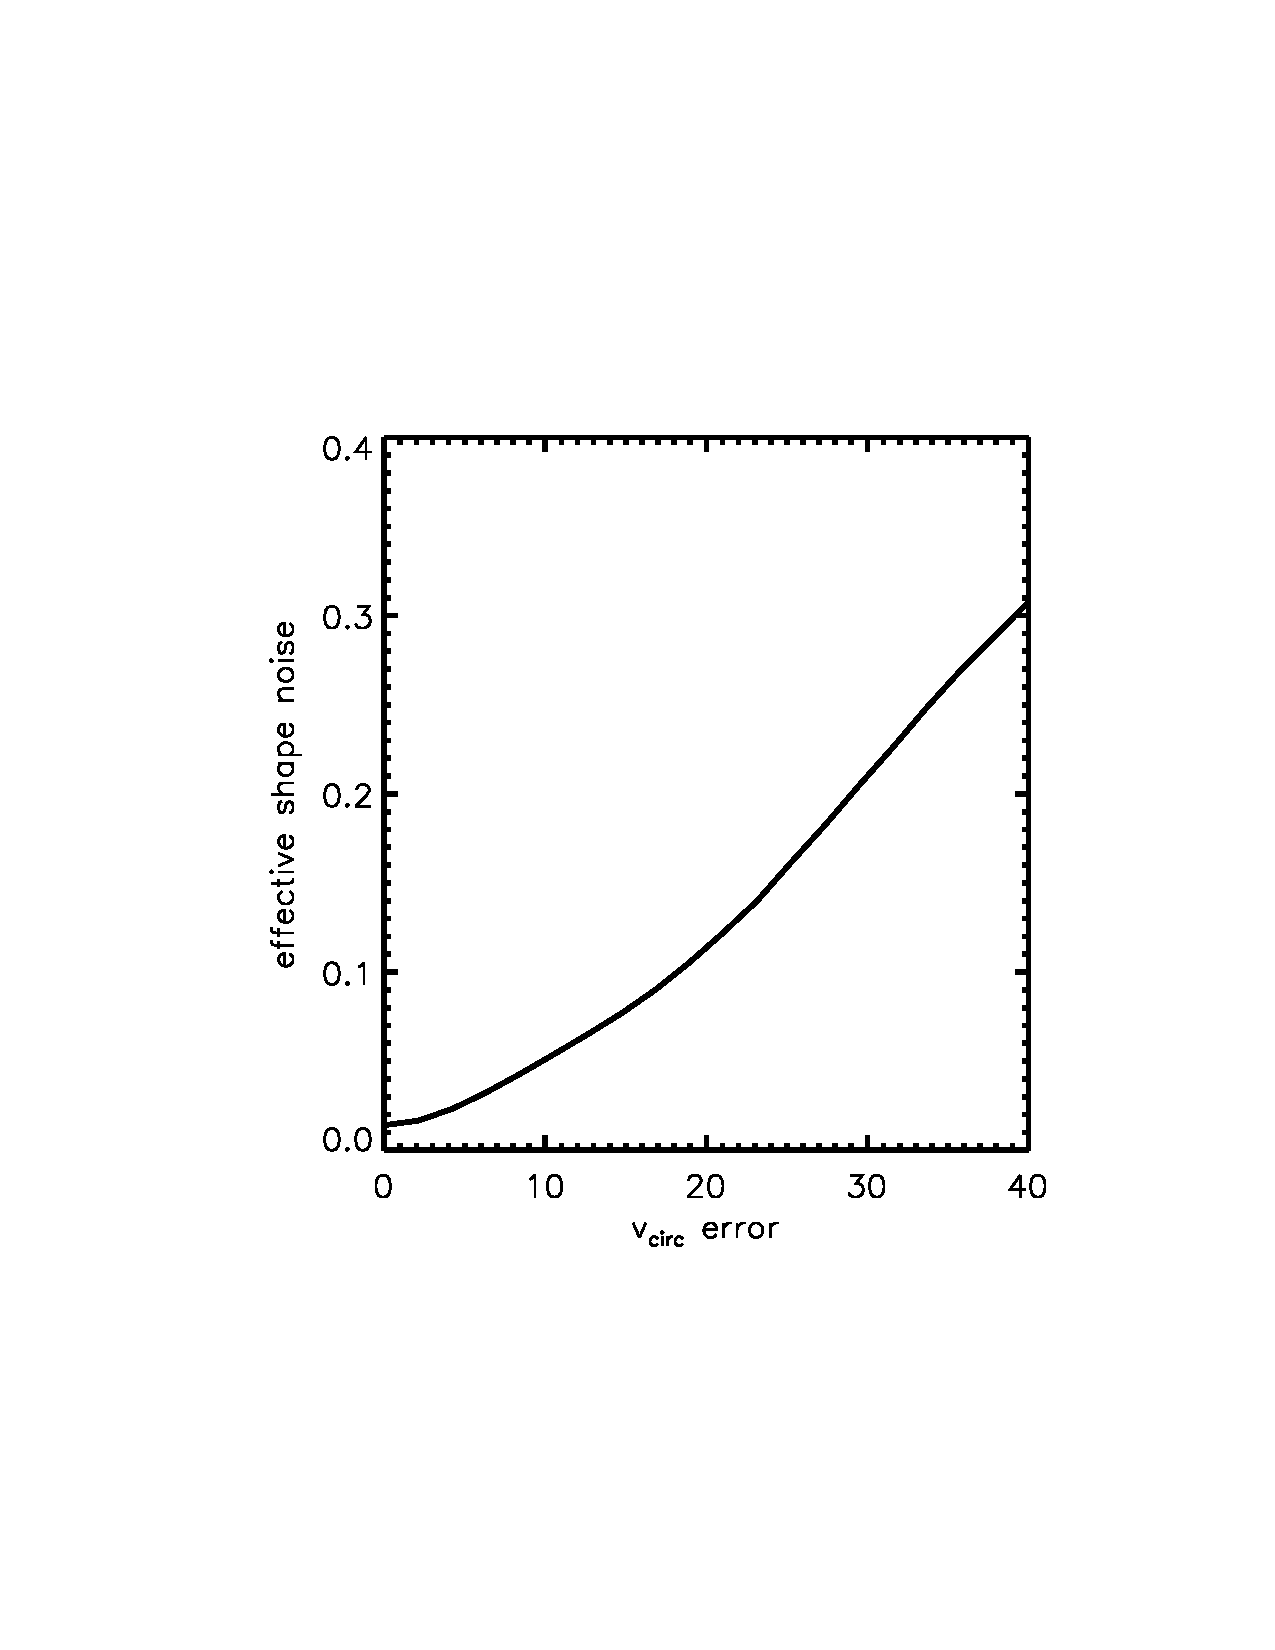
\includegraphics[width=0.45\linewidth, bb= 150 150 550 650,clip]{Plots/vcirc_error.pdf}
\caption{Effective shape noise $\sigma_{TF}$ as a  function of the
  measurement error on the disk circular velocity.}
\label{fig:shapeNoise}
\end{figure}

<<<<<<< HEAD
\subsection{Abell 2261: Precision Lensing of a Dissociative Galaxy Cluster}
The reduction in the shape noise promised by this technique will substantially improve weak lensing measurements of the mass distribution in massive galaxy clusters. One especially promising benefit is the improved ability to localize dark structures. 
=======
\bibliographystyle{apj}
\bibliography{proposal}

\section{Technical Remarks}

\subsection{Targets and Exposures}

\subsection{Backup Program}

\subsection{Supplementary Observations}

\subsection{Status of Previously Approved Keck Programs}



% The following sections are optional but highly recommended
\subsection{Path to Science from Observations}

\subsection{Technical Concerns}

\subsection{Experience and Publications}

\subsection{Resources and Publication Timescale}
>>>>>>> d9dbc942e0a1dc3bc215bd232df3eaebc4a33de1



\end{document}